\chapter{Data Reduction}
\label{cha:dataReduction}
\section{Calibration}
To actually calibrate the detectors, we use an $\alpha$-source with a known spectrum. The source are placed in the target position, and each detector is in turn placed infront of the source. 
The radioactive source used to calibrate this setup contained \isotope[148][]{Gd}, \isotope[239][]{Pu} and \isotope[244][]{Cm}. each isotope has a prominent main peak, and several sub peaks. The proprieties of which is listed in  \cref{tab:cali}.
\begin{table}[H]
	\centering
	\begin{tabular}{ll}
		Isotope & $E_\alpha \ [keV]$  \\ \hline
		\isotope[148][]{Gd}		& 3182.690         \\
		\isotope[239][]{Pu}		& 5105.5           \\
								& 5144.3           \\
								& 5156.59          \\
		\isotope[244][]{Cm}		& 5762.64          \\
								& 5804.96          \\ 
	\end{tabular}
	\caption{Decay energies for each isotope used in the calibration.}
	\label{tab:cali}
\end{table}
A typical single strip spectrum is shown on \cref{fig:singleStripExample}, where the calibrator has given an estimate of where the peaks are, illustrated by the red triangles. \cref{fig:peakExample} shows a closer look at the \isotope[244][]{Cm} peak, where the red line shows the \texttt{Calibrator}-fit over both the main peak and the sub peak. \\

\begin{figure}[h]
	\begin{subfigure}{\linewidth}
		\centering
		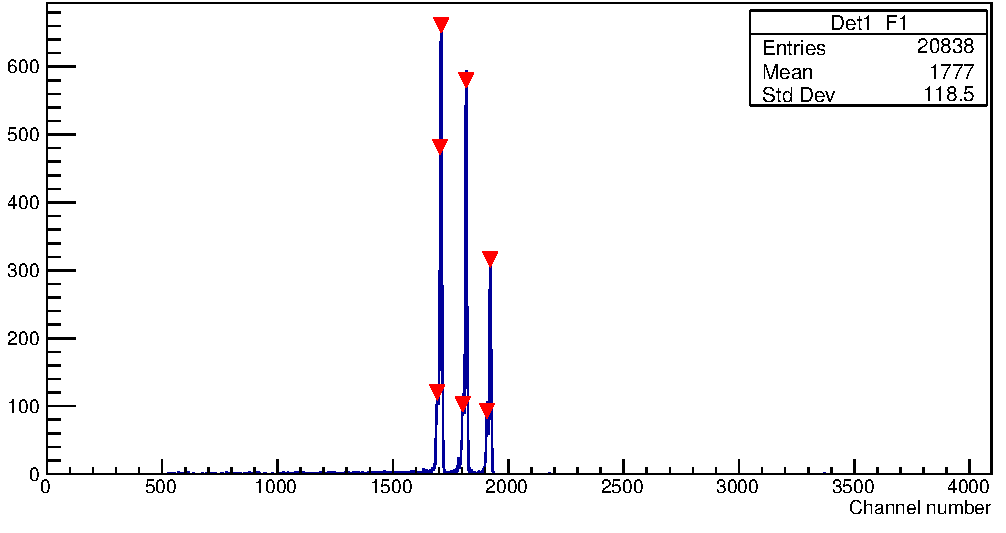
\includegraphics[width=.9\linewidth]{../figures/cali/det1f1-cropped.pdf}
		\caption{A spectrum of the calibration source, with channel number along the x-axis. The red triangles indicate the positions the \texttt{Calibrator} has guessed as the peaks.}
		\label{fig:singleStripExample}
	\end{subfigure}
	\begin{subfigure}{\textwidth}
		\centering
		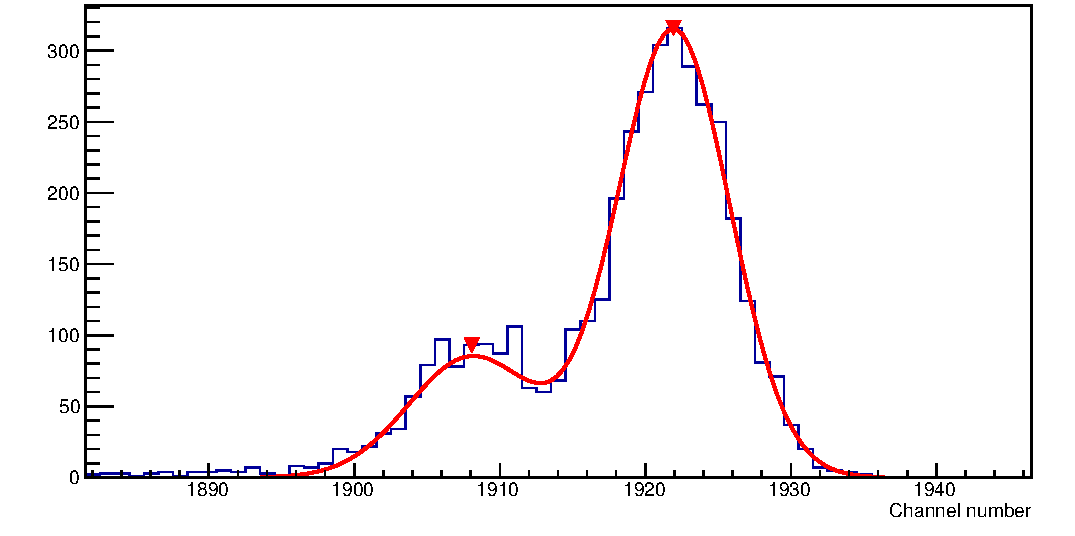
\includegraphics[width=.9\linewidth]{../figures/cali/det1f1PeakMostLeft-cropped}
		\caption{A closer look at the \isotope[244][]{Cm} peak on the above figure. The red line is a fit performed by the \texttt{Calibrator}, and the red triangles indicate the guessed peaks. }
		\label{fig:peakExample}
	\end{subfigure}
	\caption{Calibrations of detector 1}
	\label{fig:CaliExamples}
\end{figure}
